\documentclass[
	% -- opções da classe memoir --
	article,			% indica que é um artigo acadêmico
	11pt,				% tamanho da fonte
	oneside,			% para impressão apenas no recto. Oposto a twoside
	a4paper,			% tamanho do papel.
	% -- opções da classe abntex2 --
	%chapter=TITLE,		% títulos de capítulos convertidos em letras maiúsculas
	%section=TITLE,		% títulos de seções convertidos em letras maiúsculas
	%subsection=TITLE,	% títulos de subseções convertidos em letras maiúsculas
	%subsubsection=TITLE % títulos de subsubseções convertidos em letras maiúsculas
	% -- opções do pacote babel --
	english,			% idioma adicional para hifenização
	brazil,				% o último idioma é o principal do documento
	sumario=tradicional
	]{abntex2}

% ---
% Pacotes fundamentais
% ---
\usepackage{lmodern}			% Usa a fonte Latin Modern
\usepackage[T1]{fontenc}		% Selecao de codigos de fonte.
\usepackage[utf8]{inputenc}		% Codificacao do documento (conversão automática dos acentos)
\usepackage{indentfirst}		% Indenta o primeiro parágrafo de cada seção.
\usepackage{nomencl} 			% Lista de simbolos
\usepackage{color}				% Controle das cores
\usepackage{graphicx}			% Inclusão de gráficos
\usepackage[export]{adjustbox}
\usepackage{microtype} 			% para melhorias de justificação
% ---
\usepackage{amsmath}
\usepackage[backend=bibtex,style=verbose-trad2]

% ---
% Pacotes de citações
% ---
\usepackage[brazilian,hyperpageref]{backref}	 % Paginas com as citações na bibl
\usepackage[alf]{abntex2cite}	% Citações padrão ABNT
% ---

% ---
% Informações de dados para CAPA e FOLHA DE ROSTO
% ---
\titulo{Trabalho Prático de\\ Controle e Servomecanismos I}
\autor{Evandro Pulz Remon Viva\thanks{TIA: 31445721} \and Isaías Rocha Lima\thanks{TIA: 31402178}}
\local{São Paulo}
\data{2017}
% ---

% informações do PDF
\makeatletter
\hypersetup{
     	%pagebackref=true,
		pdftitle={\@title},
		pdfauthor={\@author},
    	pdfsubject={Relatório do Trabalho Prático de Controle e Servomecanismos I},
	    pdfcreator={Isaías Lima e Evandro Viva},
		pdfkeywords={controle}{laplace}{realimentação}{claude}{servos},
		colorlinks=true,       		% false: boxed links; true: colored links
    	linkcolor=blue,          	% color of internal links
    	citecolor=blue,        		% color of links to bibliography
    	filecolor=magenta,      		% color of file links
		urlcolor=blue,
		bookmarksdepth=4
}
\makeatother
% ---

% ---
% compila o indice
% ---
\makeindex
% ---

% ---
% Altera as margens padrões
% ---
\setlrmarginsandblock{3cm}{2cm}{*}
\setulmarginsandblock{3cm}{2cm}{*}
\checkandfixthelayout
% ---

% ---
% Espaçamentos entre linhas e parágrafos
% ---

% O tamanho do parágrafo é dado por:
\setlength{\parindent}{1.3cm}

% Controle do espaçamento entre um parágrafo e outro:
\setlength{\parskip}{0.2cm}  % tente também \onelineskip

% Espaçamento simples
\SingleSpacing

\begin{document}

% Seleciona o idioma do documento (conforme pacotes do babel)
%\selectlanguage{english}
\selectlanguage{brazil}

% Retira espaço extra obsoleto entre as frases.
\frenchspacing

% ----------------------------------------------------------
% ELEMENTOS PRÉ-TEXTUAIS
% ----------------------------------------------------------

%---
%
% Se desejar escrever o artigo em duas colunas, descomente a linha abaixo
% e a linha com o texto ``FIM DE ARTIGO EM DUAS COLUNAS''.
% \twocolumn[    		% INICIO DE ARTIGO EM DUAS COLUNAS
%
%---
% página de titulo
\maketitle

% resumo em português
\begin{resumoumacoluna}
 A representação da Função de Transferência de um sistema de 2ª ordem pode ser elaborada
 através de um circuito elétrico com amplificadores operacionais e elementos que armazenam
 energia, tais como capacitores e indutores. Após um semestre de aprendizados, é tempo de
 colocar o que foi visto na prática e atuar em práticas do cotidiano da Engenharia,
 modelando sistemas e elaborando soluções.

 \vspace{\onelineskip}

 \noindent
 \textbf{Palavras-chave}: controle. servomecanismos. segunda ordem. matlab. simulink.
\end{resumoumacoluna}

% ----------------------------------------------------------
% ELEMENTOS TEXTUAIS
% ----------------------------------------------------------
\textual

% ----------------------------------------------------------
% Introdução
% ----------------------------------------------------------
\section*{Introdução}
\addcontentsline{toc}{section}{Introdução}

Dada uma determinada função de transferência, podemos deduzir sua equação diferencial,
de acordo com o exemplo a seguir.

\begin{align*}
  T(s) = \frac{V(s)}{U(s)} = \frac{A}{B s^2 + C s + D} \\
  B \frac{d^2 v(t)}{dt^2} + C \frac{d v(t)}{dt} + D v(t) = A u(t)
\end{align*}

\section{Função de Trasnferência analisada e Equação Diferencial}

A partir deste raciocínio, podemos, seguindo a proposta do presente trabalho, pegar o número
de matrícula 31402178 e nos utilizar dos seus quatro últimos dígitos para elaborar uma
função de transferência qualquer, que pode agora ser determinada como:

\begin{align*}
  A &= 2 \\
  B &= 1 \\
  C &= 7 \\
  D &= 8 \\
  T(s) &= \frac{2}{s^2 + 7 s + 8}
\end{align*}

Tendo a função de transferência em mãos, doravante chamada de TF, podemos provar
de modo analítico a dedução da equação diferencial que a originou, tendo como
função de entrada um ``degrau'' e como função de saída uma tensão qualquer resultante
deste processo. Para isso, aplicamos a transformada inversa de Laplace.

\begin{align*}
  2U(s) &= (s^2 + 7s + 8)V(s) \\
  2U(s) &= s^2 V(s) + 7sV(s) + 8V(s) \\
  2u(t) &= \frac{d^2 v(t)}{dt^2} + 7\frac{d v(t)}{dt} + 8v(t) \\
\end{align*}

\section{Alguns valores notáveis}

A partir da TF, podemos calcular alguns valores notáveis, parâmetros que apresentam o funcionamento dela. São estes ${\%UP}$, ${\zeta}$, ${\omega_n}$, ${\sigma_d}$, ${\omega_d}$, ${Ts}$, ${Tp}$, ${Tr}$ e ${G(s)}$, sendo que ${\%UP}$, ${\omega_d}$ e ${Tp}$ não precisam ser calculados (dado que o comportamento da TF, como será visto, é superamortecido) e ${Ts}$, ${\zeta}$ e ${\omega_n}$ serão deduzidos mais adiante (usaremos o valor já calculado). Abaixo, a dedução dos valores, considerando realimentação unitária (${H(s) = 1}$):

\begin{align*}
  \sigma_d &= \zeta\omega_n = 3,5 \\
  \frac{G(s)}{1 + G(s)} &= \frac{2}{s^2 + 7s + 8} \\
  G(s) - \frac{2G(s)}{s^2 + 7s + 8} &= \frac{2}{s^2 + 7s + 8} \\
  G(s)(\frac{s^2 + 7s + 6}{s^2 + 7s + 8}) &= \frac{2}{s^2 + 7s + 8} \\
  G(s) &= \frac{2}{s^2 + 7s + 6}
\end{align*}

\newpage

\section{Resposta ao Degrau Unitário e Valor Final via \emph{Matlab}}

Abaixo, \emph{script} \emph{Matlab} para apresentação do mapa de pólos e zeros (que comprova o tipo de amorteciento do sistema) e para apresentação da resposta ao ``degrau'', bem como a saída para a janela de comandos, estando assinalados os valores notáveis dos gráficos.

\begin{verbatim}
  clc
  clear all
  clear space

  T = tf([2],[1 7 8]) % definição da função de transferência
  step(T) % resposta ao degrau
  figure % abertura de nova janela para o próximo gráfico
  pzmap(T) % mapa de pólos e zeros
\end{verbatim}

\begin{verbatim}

  Transfer function 'T' from input 'u1' to output ...

                     2
          y1:  -------------
               s^2 + 7 s + 8

  Continuous-time model.

\end{verbatim}

Executando o \emph{script}, obtemos os resultados apreciados nas Figuras \ref{fig:pzmap} e \ref{fig:step}.

\begin{figure}[b]
  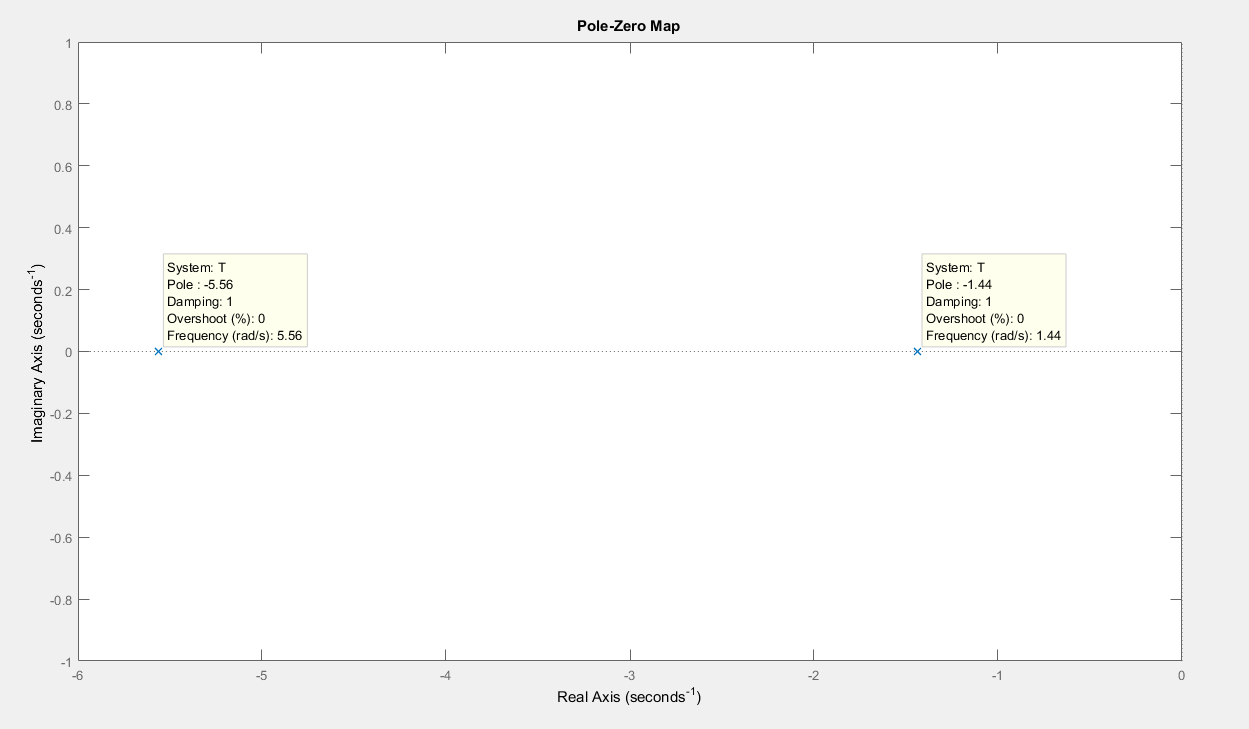
\includegraphics[width=\linewidth, center]{pzmap.png}
  \caption{Mapa de pólos e zeros da TF.}
  \label{fig:pzmap}
\end{figure}

\begin{figure}
  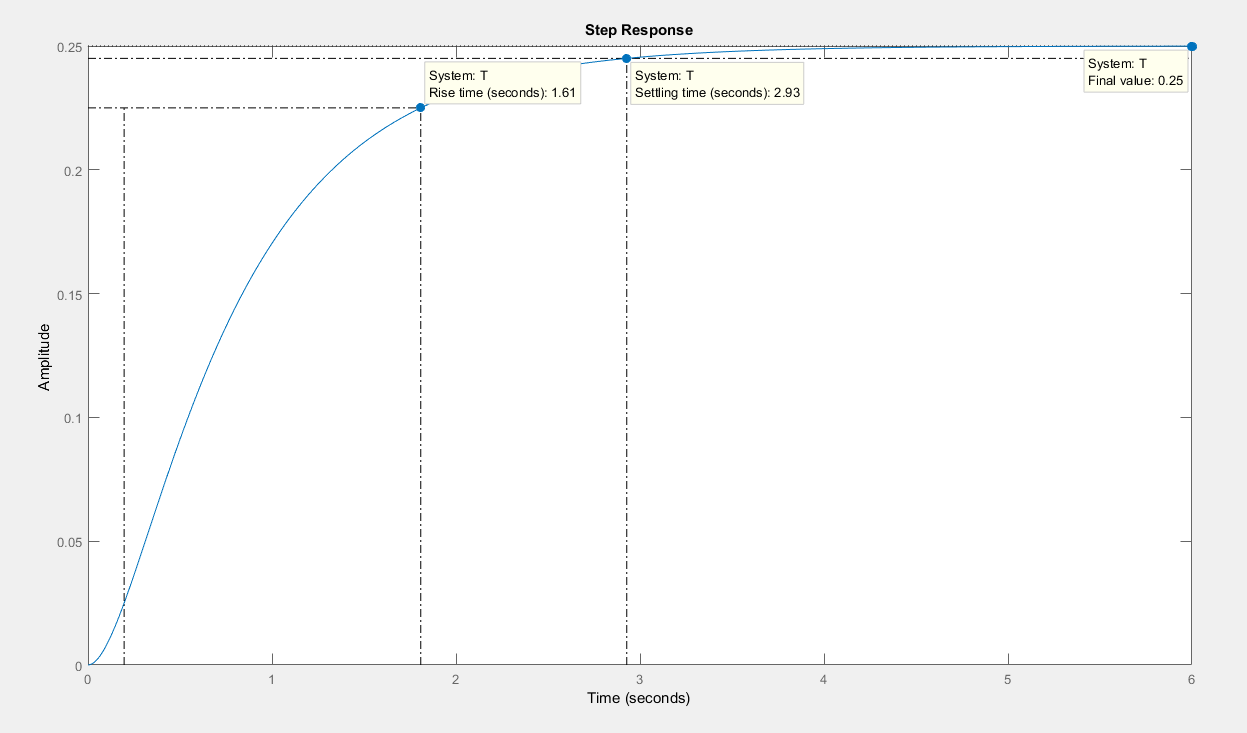
\includegraphics[width=\linewidth, center]{step.png}
  \caption{Resposta ao ``degrau'' da TF.}
  \label{fig:step}
\end{figure}

\section{Resposta ao Degrau Unitário e Valor Final \emph{Analiticamente}}

A partir dos conhecimentos desenvolvidos na disciplina de Controle e Servomecanismos I, podemos desenvolver analiticamente
o cálculo da resposta ao ``degrau'' e do valor final da FT mostrados anteriormente.

Para uma TF de segunda ordem qualquer (semelhante à colocada no início do presente documento), sabemos que:

\begin{align*}
  C &= 2\zeta\omega_n \\
  D &= \omega_n^2
\end{align*}

Sendo ${\zeta}$ a constante de amortecimento do sistema e ${\omega}$n sua frequência natural de oscilação. Também sabemos, a partir do seu mapa de pólos e zeros calculado anteriormente, que a TF possui comportamento superamortecido, não apresentando \emph{overshoot} e com pólos reais distintos no semiplano esquerdo (o que indica estabilidade).

Possuindo os valores de ${\zeta}$ e ${\omega}$, podemos calcular os parâmetros que definirão sua resposta ao ``degrau'':

\begin{align*}
  Ts &= \frac{-3}{p_1}
\end{align*}

Sendo ${Ts}$ o tempo de assentamento da TF e ${p1}$ o primeiro pólo encontrado através do \emph{script Matlab}, resultando num valor aproximado com erro de cerca de 5\%. Também podemos calcular a qual valor a TF tende quando estimulada, através da fórmula, sendo ${C(s)}$ a função de saída de um sistema qualquer:

\begin{align*}
  Cfinal = c(t\to\infty) = \lim_{s\to 0} sC(s)
\end{align*}

Abaixo, todos os valores são calculados e podem ser comparados com o apreciado anteriormente, nas simulações, substituindo os valores de ${A}$, ${B}$, ${C}$ e ${D}$ corretamente.

\begin{align*}
  \omega_n &= \sqrt{8} = 2,83 \\
  \zeta &= \frac{7}{2\omega_n} = 1,24 \\
  Ts &= 2,08 \\
  Cfinal &= \lim_{s\to 0} sC(s) = \lim_{s\to 0} sR(s)T(s) = \lim_{s\to 0} \frac{2}{s^2 + 7s + 8} = 0,25
\end{align*}

Observando todos os valores calculados, fica claro que a simulação está compatível com os valores esperados da TF, guardados as proporções e os devidos erros propagados pelo cálculo manual.

\section{Parâmetros do Circuito Elétrico Equivalente}

Além da equação diferencial, de acordo com \cite{controleessencial}, podemos deduzir um circuito elétrico que
apresente as características da FT analisada. Para isso, retomaremos a equação diferencial:

\begin{align*}
  2u(t) &= \frac{d^2 v(t)}{dt^2} + 7\frac{d v(t)}{dt} + 8v(t)
\end{align*}

E adotaremos a fórmula apresentada por \cite{controleessencial}:

\begin{align*}
  \frac{1}{R_2RC_1C_2}u(t) &= \frac{d^2 v(t)}{dt^2} + \frac{1}{R_1C_1}\frac{d v(t)}{dt} + \frac{1}{R_2R_3R_1C_2}v(t)
\end{align*}

Desenvolvendo e unindo ambas a partir das premissas de que ${C_1 = C_2 = 10 \mu F}$ e de que ${R_1 = R_2}$, temos:

\begin{align*}
  \frac{1}{R_1 10\mu} &= 7 \\
  R_1 &= R_2 = 14,3k\Omega \\
  \frac{1}{R_2R_3 100p} &= 8 \\
  800p R_2R_3 &= 1 \\
  R_3 &= 87,4k\Omega \\
  \frac{1}{R_2R 100p} &= 2 \\
  200p R_2R &= 1 \\
  R &= 350k\Omega
\end{align*}

E, assim, podemos realizar as simulações elétricas, construindo o circuito da TF no \emph{Multisim}.

\section{Simulação dos resultados através do \emph{Multisim}}

Trazendo as observações apreciadas nos itens anteriores para a prática, e usando os valores de ${R_1}$, ${R_2}$, ${R_3}$ e ${R}$ calculados, junto com a premissa de que ${C_1 = C_2 = 100nF}$, temos o circuito elétrico equivalente da TF e sua respectiva resposta no osciloscópio, através das Figuras \ref{fig:circuit} e \ref{fig:response}

\begin{figure}[h!]
  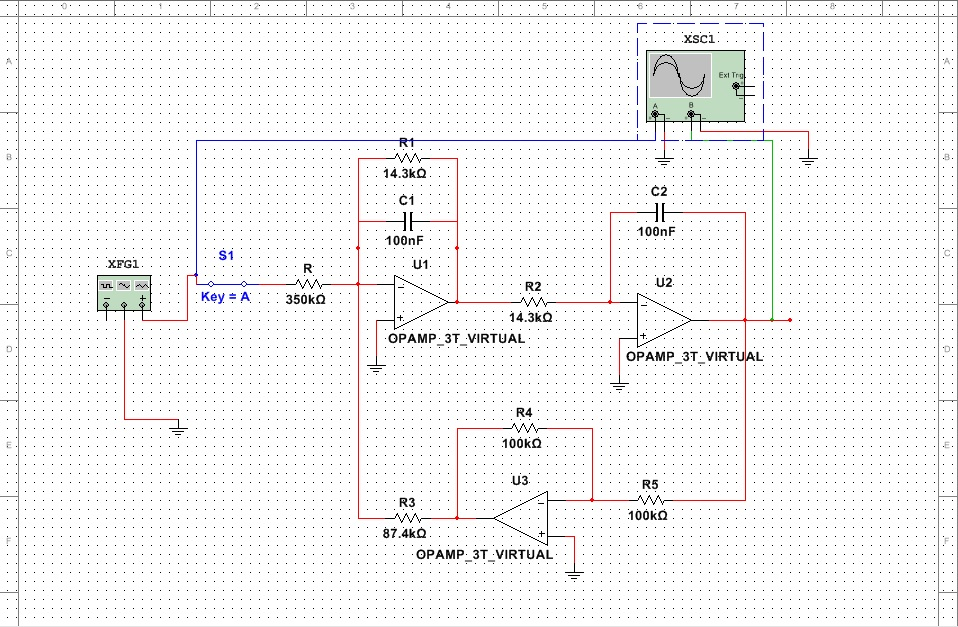
\includegraphics[width=\linewidth, center]{multisim_circuit.jpg}
  \caption{Mapa de pólos e zeros da TF.}
  \label{fig:circuit}
\end{figure}

\begin{figure}[h]
  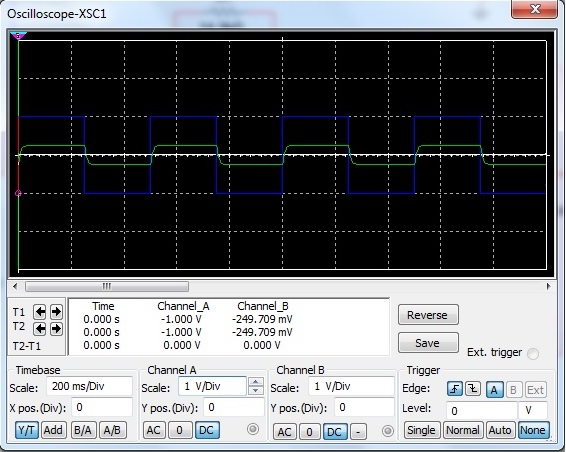
\includegraphics[width=\linewidth, center]{multisim_response.jpg}
  \caption{Mapa de pólos e zeros da TF.}
  \label{fig:response}
\end{figure}

\newpage

% ----------------------------------------------------------
% Referências bibliográficas
% ----------------------------------------------------------
\bibliography{references}

\end{document}
